\documentclass[12pt,one column]{article}
\usepackage{listings}
\usepackage{float}
\usepackage{mathtools}
\usepackage[english,russian]{babel}
\everymath{\displaystyle}
\usepackage{hyperref}
\usepackage{verbatim}
\usepackage[usenames]{color}
\usepackage{colortbl}
\usepackage{booktabs}
\usepackage{placeins}
\usepackage{longtable}
\usepackage{multirow}
\usepackage{xcolor}
\usepackage{verbatim}
\usepackage[T2A]{fontenc}
\usepackage{geometry}
\geometry{
  a4paper,
  top=25mm, 
  right=15mm, 
  bottom=25mm, 
  left=15mm
}

\begin{document}
\begin{center}
  Федеральное государственное автономное образовательное учреждение высшего образования "Национальный Исследовательский Университет ИТМО"\\ 
  Мегафакультет Компьютерных Технологий и Управления\\
  Факультет Программной Инженерии и Компьютерной Техники \\
  
\includegraphics[scale=0.2]{itm.jpg} % нужно закинуть картинку логтипа в папку с отчетом
\end{center}
\vspace{1cm}

\begin{center}
  \large \textbf{Вариант №15}\\
  \textbf{Практическая работа №5}\\
  по дисциплине\\
  \textbf{Теория вероятностей}
\end{center}

\vspace{2cm}

\begin{flushright}
Выполнил Студент  группы P32101\\
\textbf{Лапин Алексей Александрович}\\
Преподаватель: \\
\textbf{Селина Елена Георгиевна}\\
\end{flushright}

\vspace{6cm}
\begin{center}
  г. Санкт-Петербург\\
  2023г.
\end{center}
\newpage
\tableofcontents
\newpage
\section{Текст задания:}
Каждый студент получает выборку из 20 чисел. Необходимо определить следующие статистические характеристики: вариационный ряд, экстремальные значения и размах, оценки математического ожидания и среднеквадратического отклонения, эмпирическую функцию распределения и её график, гистограмму и полигон приведенных частот группированной выборки. Для расчета характеристик и построения графиков нужно написать программу на одном из языков программирования. Листинг программы и результаты работы должны быть представлены в отчете по практической работе.\\
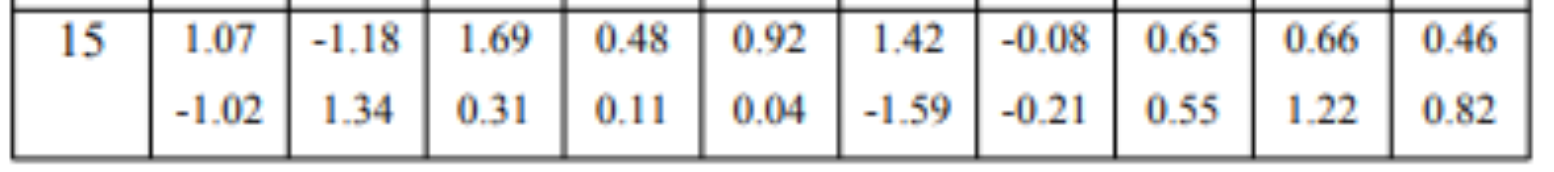
\includegraphics[width=\textwidth]{img/task.png}
\section{Листинг программы}
\lstset{
    language=Python,
    basicstyle=\ttfamily,
    keywordstyle=\bfseries\color{orange},
    showstringspaces=false,
    showtabs=false,
    stringstyle=\color{blue}\ttfamily,
}
\lstinputlisting[language=Python]{main.py}

\section{Результаты работы} 
\begin{verbatim}
    ========[Variation series]========================
    [-1.59, -1.18, -1.02, -0.21, -0.08, 0.04, 0.11, 0.31, 0.46, 0.48,
     0.55, 0.65, 0.66, 0.82, 0.92, 1.07, 1.22, 1.34, 1.42, 1.69]
    ========[Characteristics of the variation series]========
    maximum value:  1.69
    minimum value:  -1.59
    range:  3.28
    expected value: 0.383
    standard deviation: 0.8547
    ========[Empirical distribution function]========
    x < -1.59:      F(x) = 0.0
    -1.59 <= x < -1.18:     F(x) = 0.05
    -1.18 <= x < -1.02:     F(x) = 0.1
    -1.02 <= x < -0.21:     F(x) = 0.15
    -0.21 <= x < -0.08:     F(x) = 0.2
    -0.08 <= x < 0.04:      F(x) = 0.25
    0.04 <= x < 0.11:       F(x) = 0.3
    0.11 <= x < 0.31:       F(x) = 0.35
    0.31 <= x < 0.46:       F(x) = 0.4
    0.46 <= x < 0.48:       F(x) = 0.45
    0.48 <= x < 0.55:       F(x) = 0.5
    0.55 <= x < 0.65:       F(x) = 0.55
    0.65 <= x < 0.66:       F(x) = 0.6
    0.66 <= x < 0.82:       F(x) = 0.65
    0.82 <= x < 0.92:       F(x) = 0.7
    0.92 <= x < 1.07:       F(x) = 0.75
    1.07 <= x < 1.22:       F(x) = 0.8
    1.22 <= x < 1.34:       F(x) = 0.85
    1.34 <= x < 1.42:       F(x) = 0.9
    1.42 <= x < 1.69:       F(x) = 0.95
    1.69 <= x:      F(x) = 1.0
\end{verbatim}
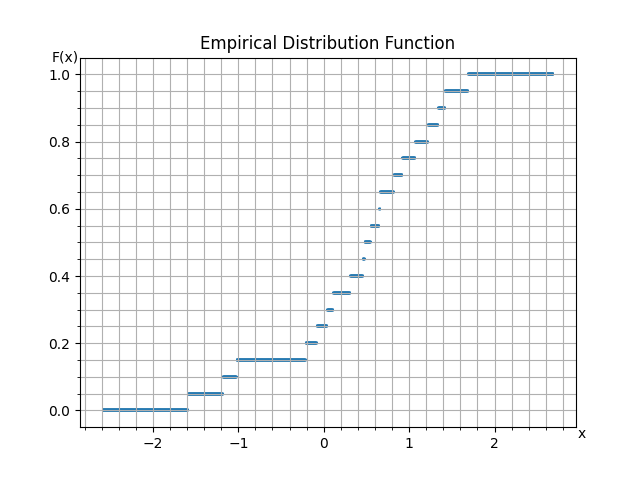
\includegraphics[width=\textwidth]{img/plot1.png}
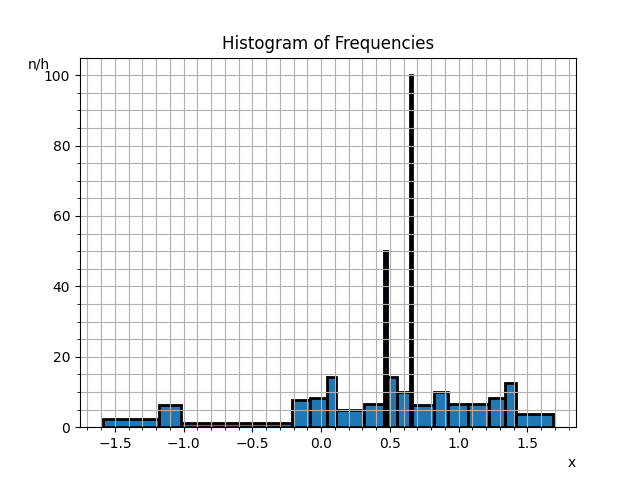
\includegraphics[width=\textwidth]{img/plot2.png}
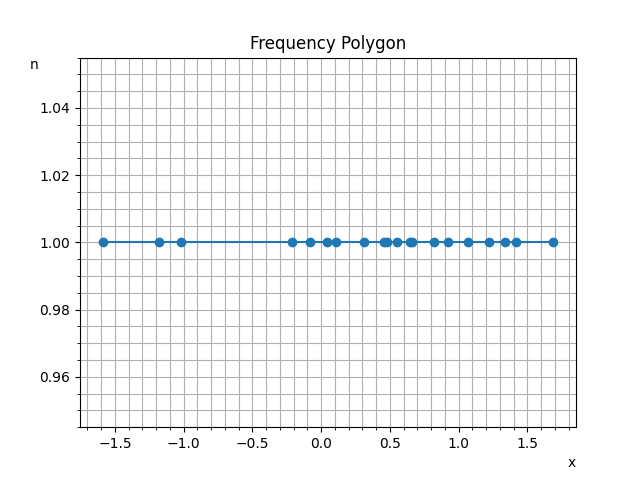
\includegraphics[width=\textwidth]{img/plot3.png}

\section{Выводы}
В процессе выполнения данной практической работы я написал программу на языке программирования Python, которая позволяет рассчитывать основные статистические характеристики выборки и строить графики эмпирической функции распределения, гистограммы и полигон.\\

В результате выполнения данной работы я узнал, как использовать стандартные библиотеки Python для работы с математическими функциями и графиками, а также научился применять методы статистики для решения задач.


\end{document}